\setcounter{Exercise}{4}
\begin{Exercise}
	This problem is quite simple.
	\begin{enumerate}
		\item $4c=5s$ where $c$ is the number of people of ordered cheesecake, and $s$ the number who ordered strudel.
		\item $6s = p$ where $p, s$ is the number of professors and students respectively.
	\end{enumerate}
\end{Exercise}

\begin{Exercise}
Let the height of the crossing be denoted $h$, and let the left pole be of height $x$ and the right pole of height $y$.
We seek to establish a relationship between the three variables, which we will do using similar triangles.

Let the distance between the bases of the two pole be denoted $c = c_1 + c_2$ where $c_1$ is the segment from the left pole
to the crossing, and $c_2$ the segment from the right pole to the crossing. 
We can then write the following expression from viewing the similar triangles:
\begin{align}
	\frac{c_2 x}{c_1 + c_2} = \frac{h}{c_2}
\end{align}
Similarly for the other variable:
\begin{align}
	\frac{c_1 y}{c_1 + c_2} = \frac{h}{c_1}.
\end{align}

Combining the two and solving for $\frac{x}{y}$, we have $\frac{x}{y} = \frac{c_1}{c_2}$. 
Now:
\begin{align}
	h &= \frac{c_2 x}{c_1 + c_2} \\
	&= \frac{x}{\frac{c_1}{c_2} + 1} \\
	&= \frac{x}{\frac{x}{y} + 1} \\
	&= \frac{xy}{x+y}
\end{align} \qed
\end{Exercise}

\begin{Exercise}
	(A bit lazy with the figures for this one, so I'll try to explain this with words).
	Note that there are probably many solutions to this.
	Let $k$ be the length of the right triangle that is opposite angle $\theta$. 
	We can express $k$ as a $\tan(\theta) = \frac{k}{L}$. 

	Since we know the width of the paper, the remaining length is $8-k$. 
	The hypotenuse of the right triangle at the bottom left corner of figure 1.17 is of length $k$ also, as it's simply folded up.
	Only one thing remains, which is that the angle for the right triangle at the bottom is of $2\theta$, by simply tallying up the angles.

	Finally, we have the expression:
	\begin{align}
		\cos(2\theta) = \frac{k}{8-k} \\
		\frac{8\cos(2\theta)}{1 + \cos(2\theta)} &= k \\
		\frac{8\cos(2\theta)}{1 + \cos(2\theta)} &= k \\
		\frac{8\cos(2\theta)}{1 + \cos(2\theta)} &= L\tan(\theta) \\
		L &= \frac{1}{\tan(\theta)}\frac{8\cos(2\theta)}{1 + \cos(2\theta)}
	\end{align}
	One can simplify this more, but the main goal is accomplished.	\qed
\end{Exercise}

\begin{figure}[h]
	\centering
	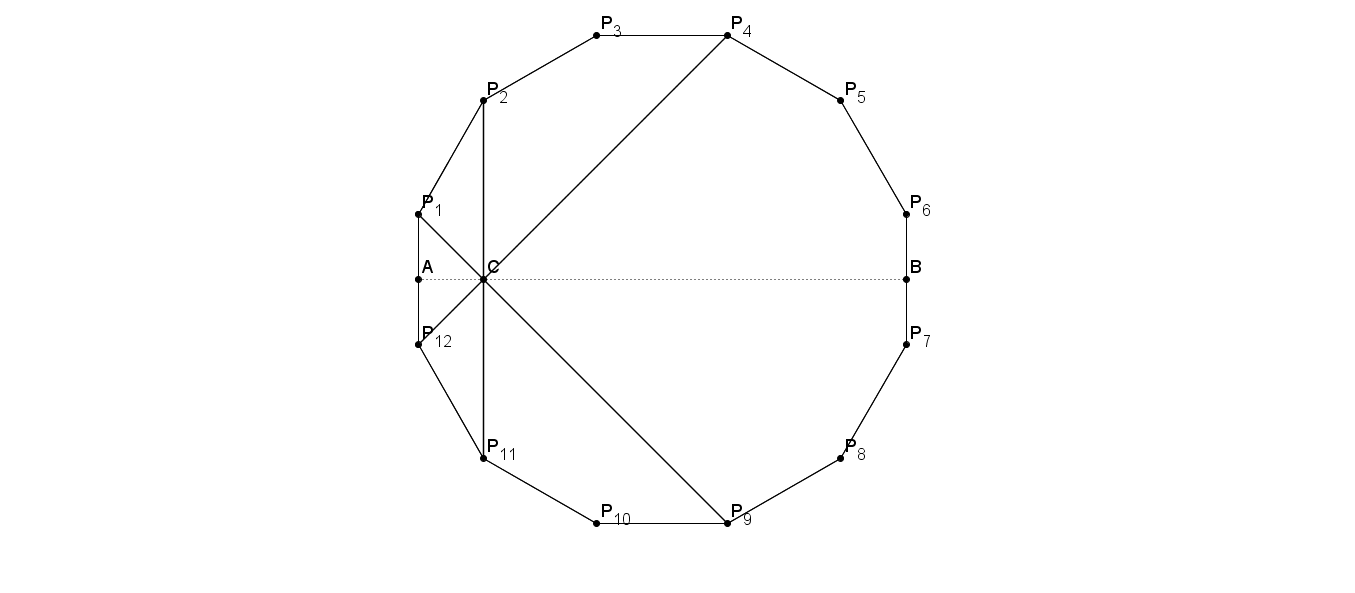
\includegraphics[width=1.2\textwidth]{./figures/chpt1/1_5_8.png}
	\caption{Exercise 1.5.8}
	\label{fig:1_5_8}
\end{figure}

\begin{Exercise}
	We see from figure~\ref{fig:1_5_8} that indeed they are concurrent, but we need to prove this rigorously.

	The angle of $CP_1P_{12} = P_{12}P_1C = 45^{\circ}$ by looking at polygons created by the diagonals itself and the dodecagon.
	If we let the side length of the dodecagon be $x$, then $P_1P_9$ and $P_4P_{12}$ intersects at exactly $x/2$ distance away from the segment $P_1P_{12}$ by the properties of right triangle ($P_1P_{12}C$ is the special right triangle).

	It is obvious that $P_2P_{11}$ creates a trapezoid with angles 150 and 30. 
	Since we have the angle, we can now find the height of the trapezoid, which is exactly $x/2$ as predicted (using $\sin 30^{\circ}$).

	One has to tie this proof a bit tighter for the Putnam exam though by proving the diagonals first intersect line $AB$,
	\footnote{a symmetry argument should do here} but
	this is a good enough sketch I think. \qed
\end{Exercise}

\begin{Exercise}
	\begin{enumerate}
		\item Average rate by definition means the total distance over total time. 
		The key point to note is that the time spent driving from point $A$ to $B$ will be \emph{more} then the other way around, 
		since the speed is slower. 
		Henyce, the average rate is less than 50 miles per hour. 

		Algebraically, let $x$ be the distance between $A$ and $B$.
		We have the following:
		\begin{align}
			s &= \frac{d}{t} \\
			&= \frac{2x}{\frac{x}{40} + \frac{x}{60}} \\
			&= \frac{2(2400)}{40 + 60}
		\end{align}
		and we see that it's the harmonic average of the two speeds. 
		The cool thing is that the distance doesn't matter at all! \qed

		\item Of course, we see physically that the two must equal, but we should do this algebraically.
		We'll do this the hard way, by keeping both the amounts of liquid and the volume of the spoon as variables (instead of scaling the spoon volume to 1).

		Let $V$ be the volume of the coffee (and the cup of cream), then let $x$ be the volume of the spoon. 
		The initial scoop will result in $V$ coffee and $x$ cream in the coffee cup and $V-x$ cream in the cream cup.
		Now the scoop from the coffee cup will contain $x \cdot \frac{x}{V+x}$  amount of cream, and $x \cdot \frac{V}{V+x}$ amount of coffee.

		This means that the final amount of cream left in the coffee cup is $x - x\cdot \frac{x}{V+x}$, while the total amount of 
		coffee in the coffee cup is $0 + x\cdot \frac{V}{V+x}$. 
		One can verify easily that they are equal. \qed

		\item Let the radius of the Earth in feet be $R$, then the original length of the rope is $2\pi R$.
		Extending that string by 6 feet will result in the new length to be $2\pi R + 6$. 

		We wish to find the new radius which have that value as its circumference; this is done by dividing by $2\pi$.
		Thus, the string is lifted by $\frac{6}{2\pi}$ total feet, which is around 1 foot and greater than an inch. \qed
	\end{enumerate}
\end{Exercise}
